\documentclass{beamer}

\graphicspath{{../images/}{../../images}}

\usepackage{theme/beamerthemehbrs}

\usepackage[utf8]{inputenc}
\usepackage{amsmath}
\usepackage{amsfonts}
\usepackage{amssymb}
\usepackage{graphicx}
\usepackage{subcaption}
\usepackage{ragged2e}  % `\justifying` text
\usepackage{booktabs}  % Tables
\usepackage{multirow}
\usepackage{tabularx}
\usepackage[export]{adjustbox}
\usepackage{array}
\newcolumntype{L}[1]{>{\raggedright\let\newline\\\arraybackslash\hspace{0pt}}p{#1}}
\newcolumntype{C}[1]{>{\centering\let\newline\\\arraybackslash\hspace{0pt}}p{#1}}
\newcolumntype{R}[1]{>{\raggedleft\let\newline\\\arraybackslash\hspace{0pt}}p{#1}}
\usepackage{amsmath}
\usepackage{amssymb}
\usepackage{dsfont}
\usepackage{url}       % `\url
\usepackage{listings}  % Code listings
\usepackage[T1]{fontenc}
\usepackage{hyperref}

% biblatex
\usepackage[backend=biber,natbib=true]{biblatex}
\addbibresource{../RnD.bib}
\renewcommand*{\bibfont}{\tiny}

% metadata
\author[Nguyen]{Minh Nguyen}
\title{Research and Development Project}
\subtitle{Learning Grasp Evaluation Models Using Synthetic 3D Object-Grasp Representations}
\institute[HBRS]{Hochschule Bonn-Rhein-Sieg}
\date{\today}

\begin{document}
{
\begin{frame}
\titlepage
\end{frame}
}

%%%%%%%%%%%%%%%%%%%%%%%%%%%%%%%%%%%%%%%%
\section{Introduction}
\begin{frame}{Use Case}
    \framesubtitle{Robocup@Home}%
    \begin{block}{Problem}
        Make Lucy grasp robustly
    \end{block}
    \begin{columns}[onlytextwidth]
        \column{.5\textwidth}
        \begin{figure}[b]
            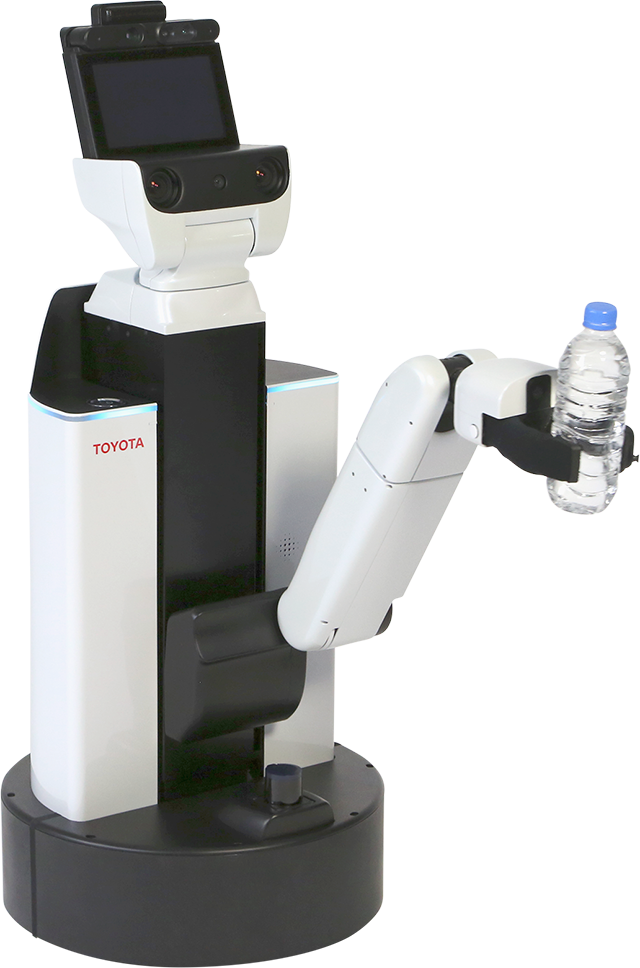
\includegraphics[width=0.45\textwidth]{hsr_stock_photo}
            \caption{Human Support Robot from Toyota.}
        \end{figure}
        \column{.45\textwidth}
        \begin{figure}[b]
            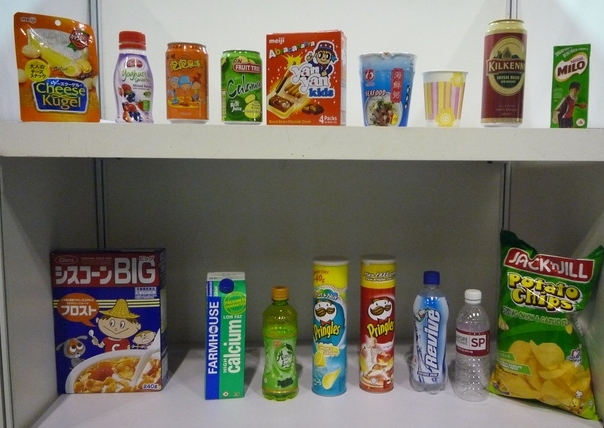
\includegraphics[width=\textwidth]{robocup_typical_objects}
            \caption{Typical objects in the Robocup@Home competition \cite{robocupRulebook2018}.}
        \end{figure}
    \end{columns}
\end{frame}

\begin{frame}{Motivation}
    \framesubtitle{Current Solution - MoveIt grasp planner}%
    A randomized planner will do inexplicable things!
    \begin{figure}[b]
        \centering
        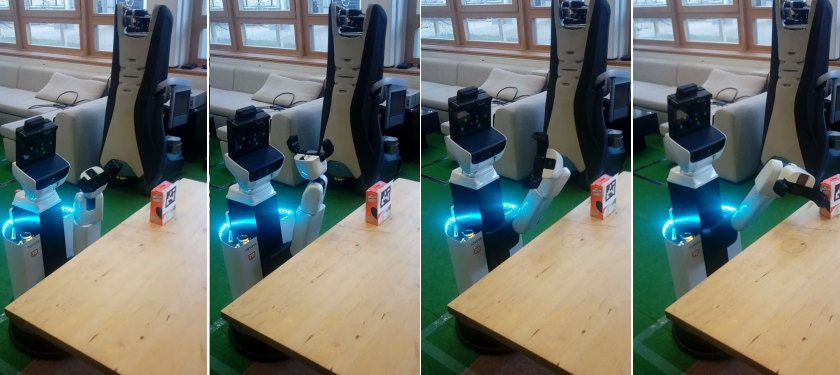
\includegraphics[width=\linewidth]{grasp_moveit_fail}
        \caption{MoveIt! failing to plan a simple grasp.}
    \end{figure}
\end{frame}

\begin{frame}[label=grasp_aspects]{Robotic Grasping Overview}
    \framesubtitle{Generating Grasp Hypotheses}
    \begin{figure}[t]
        \centering
        \begin{overprint}
            \onslide<1>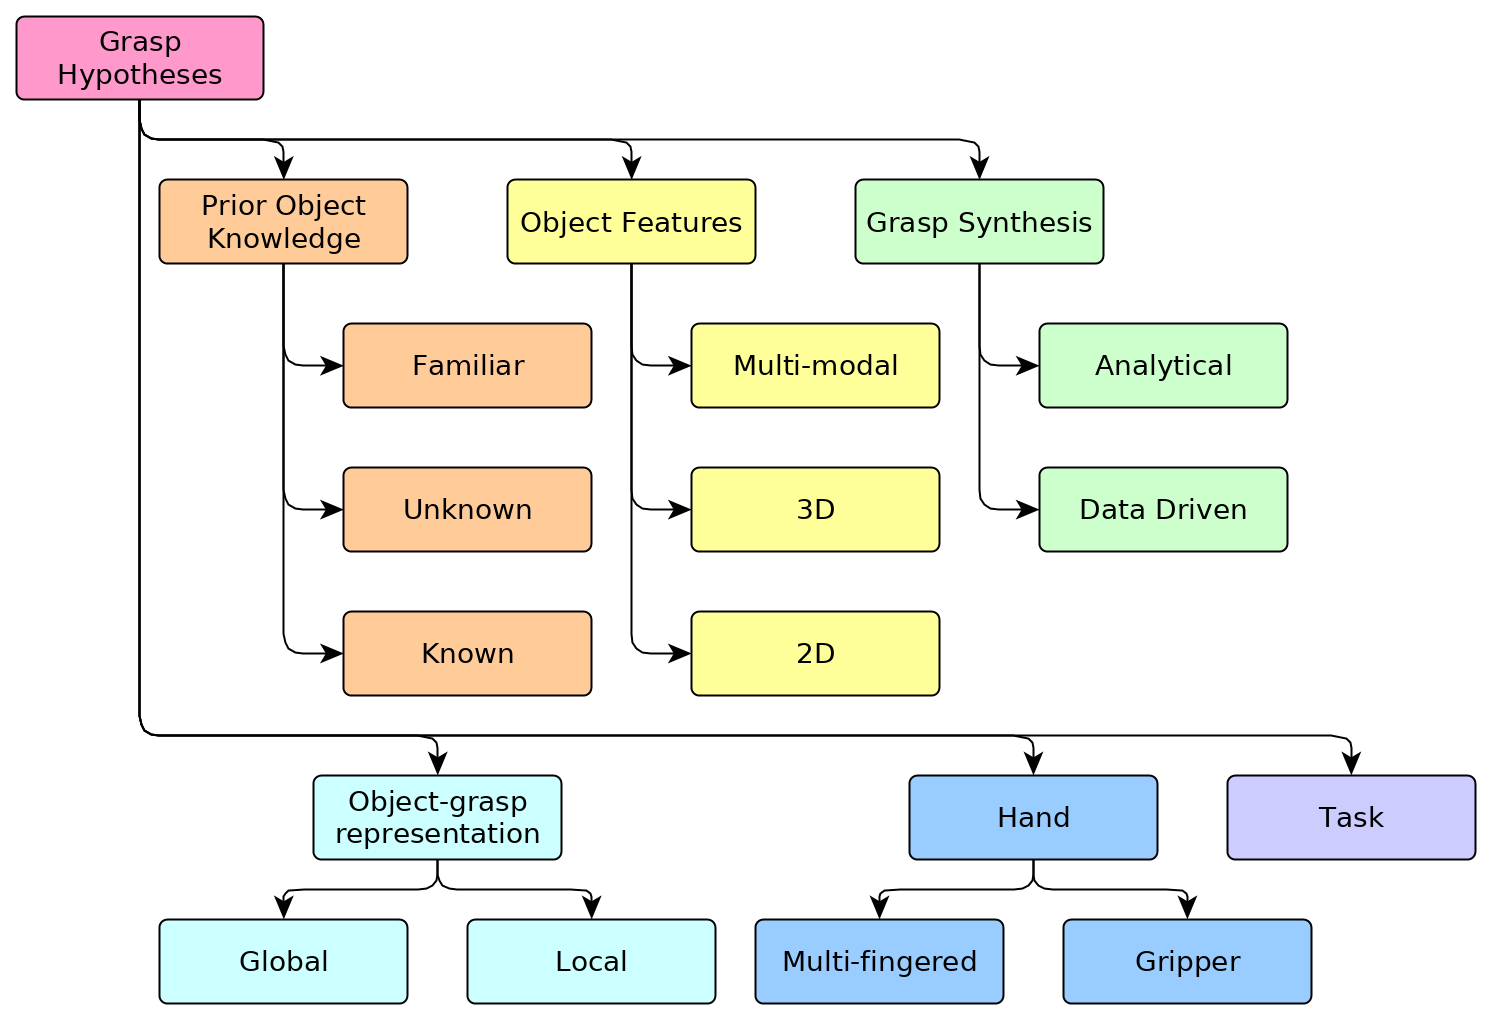
\includegraphics[width=0.85\linewidth]{bohg14-grasp_synthesis_mind_map}
            \onslide<2>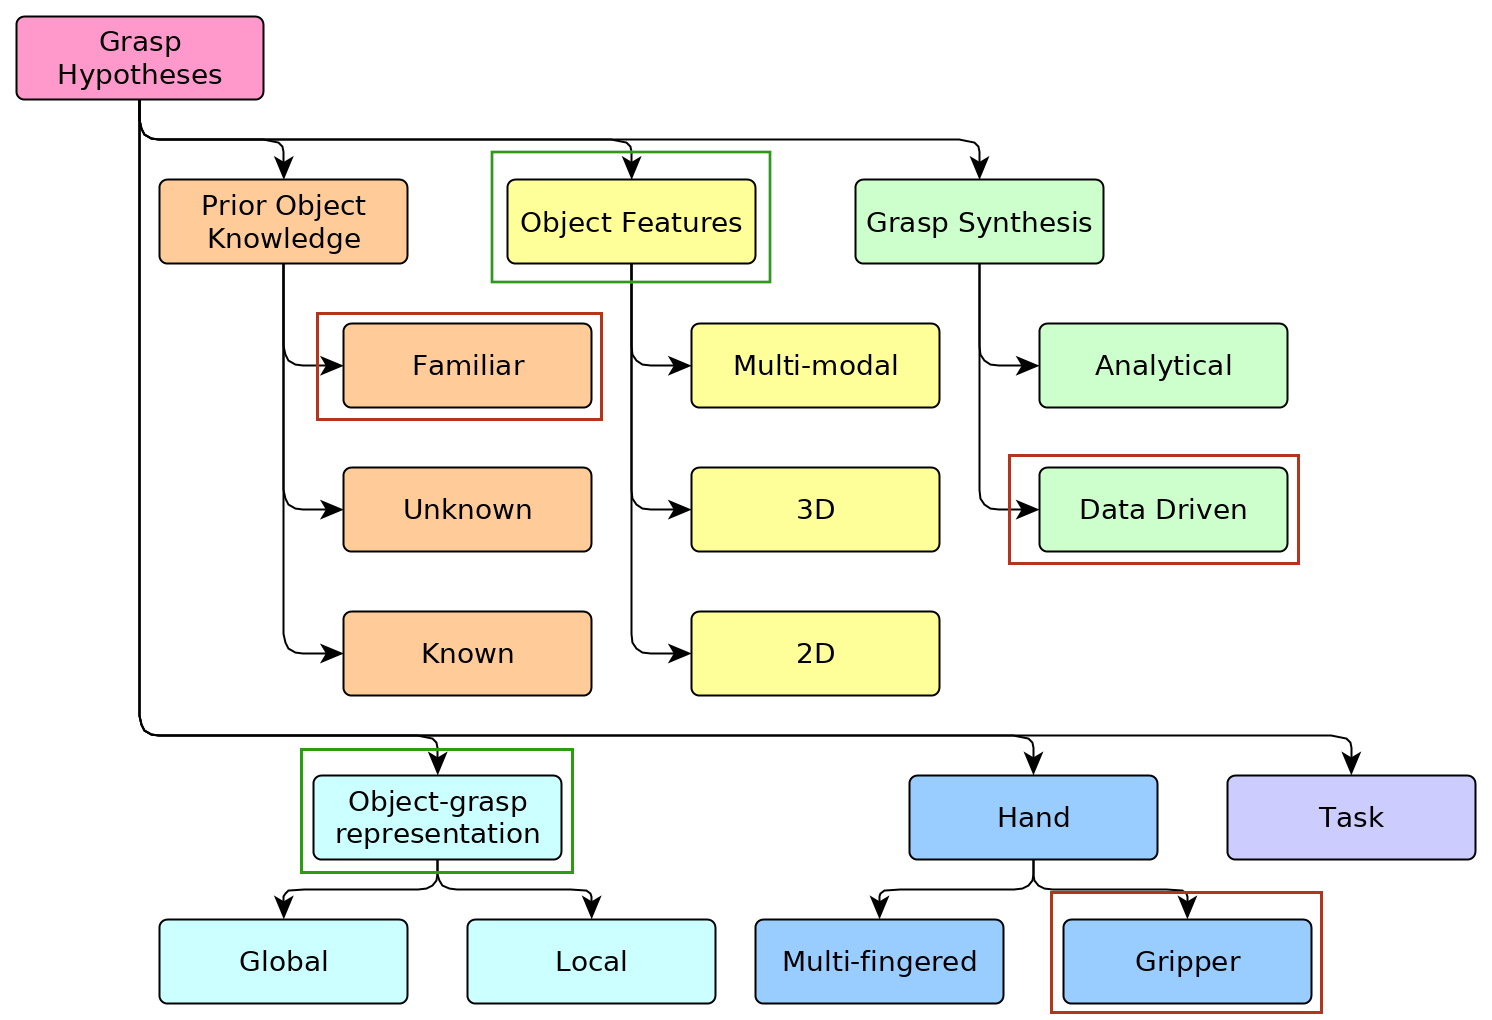
\includegraphics[width=0.85\linewidth]{bohg14-grasp_synthesis_mind_map_marked}
        \end{overprint}
        \caption{Aspects which may influence generation of grasp hypotheses \cite{Bohg2014}.}
    \end{figure}
\end{frame}

\begin{frame}{Analytical versus Empirical}
    \framesubtitle{Why not analytical grasp synthesis?}
    \begin{exampleblock}{Quick review}<1->
        \begin{itemize}
            \item \emph{Analytical grasp synthesis} consider the mechanical properties of the contact
                points \cite{Roa2015, Sahbani2012}
            \item \emph{Data-driven methods} rely on some form of grasp experience: \textit{human demonstration},
                        \textit{labeled data}, or \textit{trial-error} \cite{Bohg2014}
        \end{itemize}
    \end{exampleblock}

    \begin{exampleblock}{Shortcomings - Analytical Grasp Synthesis}<2->
        \begin{itemize}
            \item Rely on knowledge of the object's geometry, which can be inaccurate or unavailable in real
                  environments
            \item Best grasps according to analytical metrics may not be most robust grasps \cite{WeiszAllen2012}
        \end{itemize}
    \end{exampleblock}
\end{frame}

\begin{frame}{Empirical Grasp Synthesis}
    \begin{exampleblock}{Shortcomings - Empirical Grasp Synthesis}<1->
        \begin{itemize}
            \item Data collection is costly and time consuming!
            \item However, it is possible to synthesize data for training a grasp evaluation model.
        \end{itemize}
    \end{exampleblock}

    \begin{exampleblock}{Aspects important to training a grasp evaluation model}<2->
        \begin{itemize}
            \item \emph{Object-grasp representation}: how to capture the gripper-object relation in perceptual data
            \item \emph{Feature extraction and learning method}: how to use the captured representation so the model
                can learn efficiently, and which model will learn well
            \item \emph{Dataset generation}: how to synthesize and label data
        \end{itemize}
    \end{exampleblock}
\end{frame}

\begin{frame}{Empirical Grasp Synthesis}
    \begin{table}[!t]
        \tiny
        \def\arraystretch{1.2}
        \begin{tabularx}{\linewidth}{L{0.05\linewidth}C{0.39\linewidth}L{0.28\linewidth}L{0.28\linewidth}}
            Method & Object-grasp\linebreak representation & Feature extraction \& learning model & Data generation \\
            \toprule
            \cite{jiang2011}    & 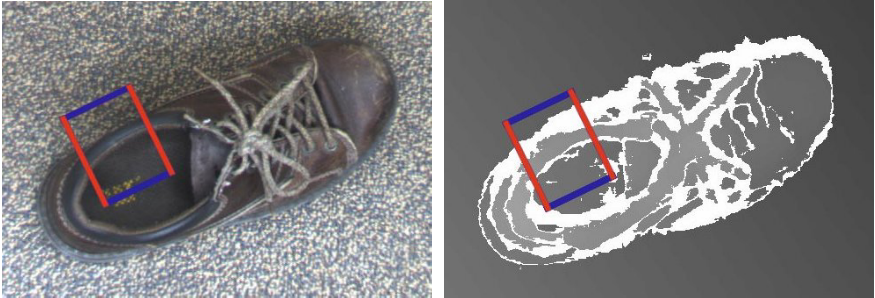
\includegraphics[scale=0.09,valign=t]{jiang_et_al-2011-grasp_representation}
                                & Histogram of hand-crafted filters; \linebreak Model: SVM.
                                & Rectangles manually \linebreak annotated. \\
            \cite{lenz2015}     & 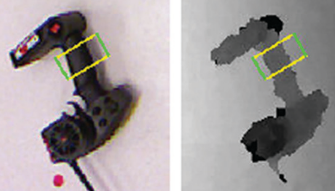
\includegraphics[scale=0.16,valign=t]{lenz_et_al-2015-grasp_representation}
                                & Auto-encoders to initialize weights, structured regularization to combine depth
                                  and RGB data; \linebreak Model: MLP.
                                & Extension of the \linebreak dataset from \cite{jiang2011} \linebreak (above).\\
            \cite{Kappler2015}  &
                        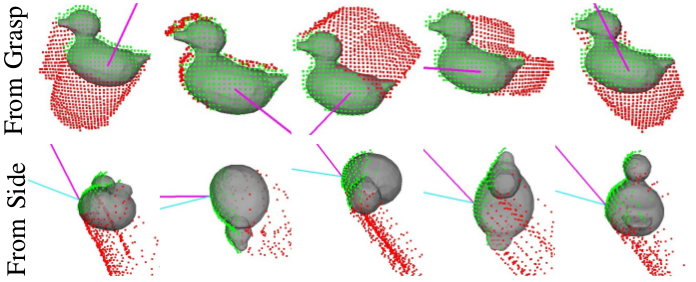
\includegraphics[scale=0.16,valign=t]{kappler_et_al-2015-fig8-local_shape_diff_viewpoints}
                                & RGB rendering of ``template grids''; \linebreak Model: LeNet CNN
                                & Quality of grasps are \linebreak calculated in simulation \linebreak for object
                                  meshes, \linebreak verified via crow-sourcing. \\
            \cite{Gualtieri2016}& 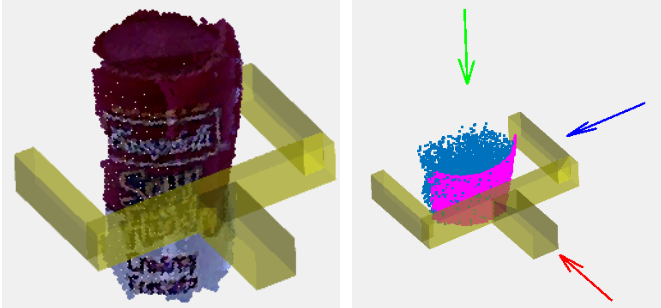
\includegraphics[scale=0.1,valign=t]{Gualtieri_et_al-2016-grasp_representation}
                                & Filters of cuboid regions projected onto 3 orthogonal planes, creating 15 channels;
                                  \linebreak Model: LeNet CNN.
                                & Quality of grasps are \linebreak calculated for object \linebreak meshes using
                                  force-closure \\
            \cite{mahler2017}   & 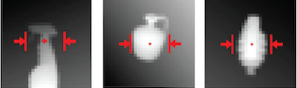
\includegraphics[scale=0.22,valign=t]{mahler_et_al-2017-grasp_representation}
                                & Depth images cropped and aligned to gripper; \linebreak Model: CNN combined
                                  with single-layer NN.
                                & Quality of grasps are \linebreak calculated for object \linebreak meshes using a
                                  variant of $ \epsilon $-metric from \cite{WeiszAllen2012} \\
            \bottomrule
        \end{tabularx}
        \caption{\tiny Five recent empirical approaches to grasp quality prediction which synthesize data}
        \label{table:grasp_approaches}
    \end{table}
\end{frame}

\begin{frame}{Dex-Net 2.0 and GQCNN}
    \begin{figure}[b]
        \centering
        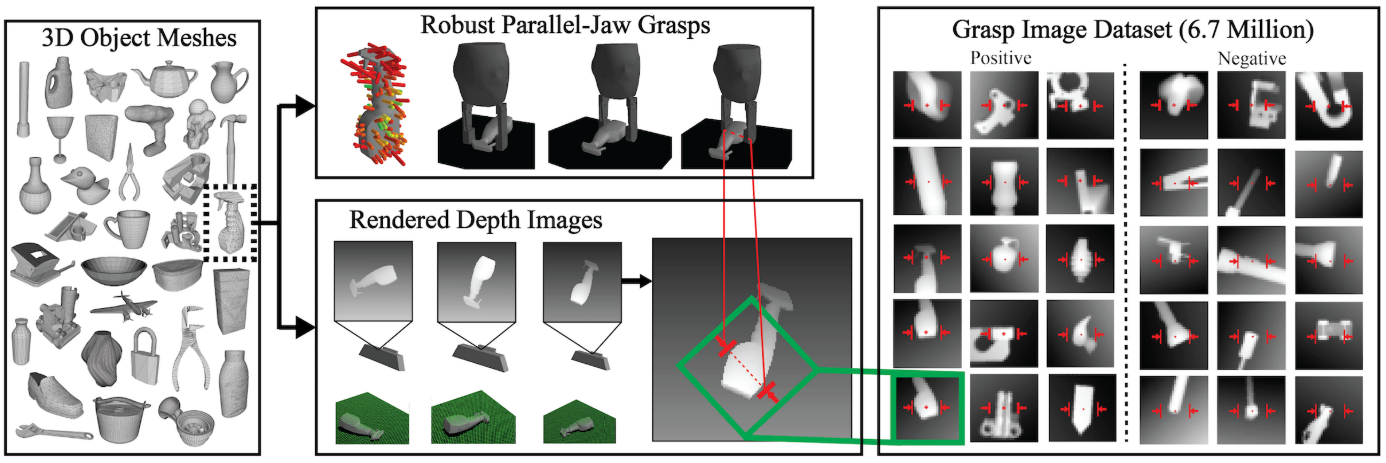
\includegraphics[width=0.9\linewidth]{mahler_et_al-2017-fig3}
        \caption{Dex-Net 2.0 pipeline for dataset generation \cite{mahler2017}}
    \end{figure}
    \begin{itemize}
        \item Labeling is done by applying analytical grasp metrics to candidates in simulation
        \item Generated data is used to train a Grasp Quality Convolutional Neural Network (GQ-CNN) to predict grasp
            quality and distance from gripper
    \end{itemize}
\end{frame}

%%%%%%%%%%%%%%%%%%%%%%%%%%%%%%%%%%%%%%%%%
\section{Methodology}
\begin{frame}{Grasping software pipeline}
\framesubtitle{Object detection -- Previous implementation}
    \begin{figure}[b]
        \centering
        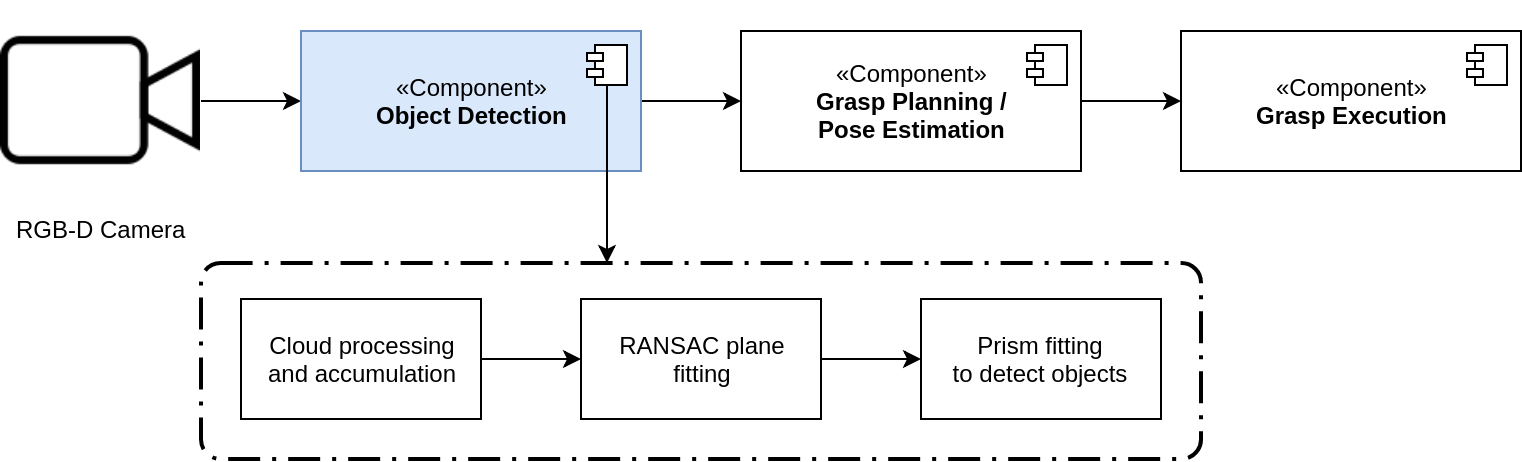
\includegraphics[width=0.8\linewidth]{grasp_pipeline_old_perception}
        \caption{Previous pipeline for object grasping.}
    \end{figure}
    \begin{exampleblock}{Challenges}
        \begin{itemize}
            \item New robot with closed-source components
            \item Previous object detection algorithm was unreliable and not suited for domestic objects
        \end{itemize}
    \end{exampleblock}
\end{frame}

%%%%%%%%%%%%%%%%%%%%%
\begin{frame}{Grasping software pipeline}
\framesubtitle{Object detection -- New architecture}
    \begin{figure}[b]
        \centering
        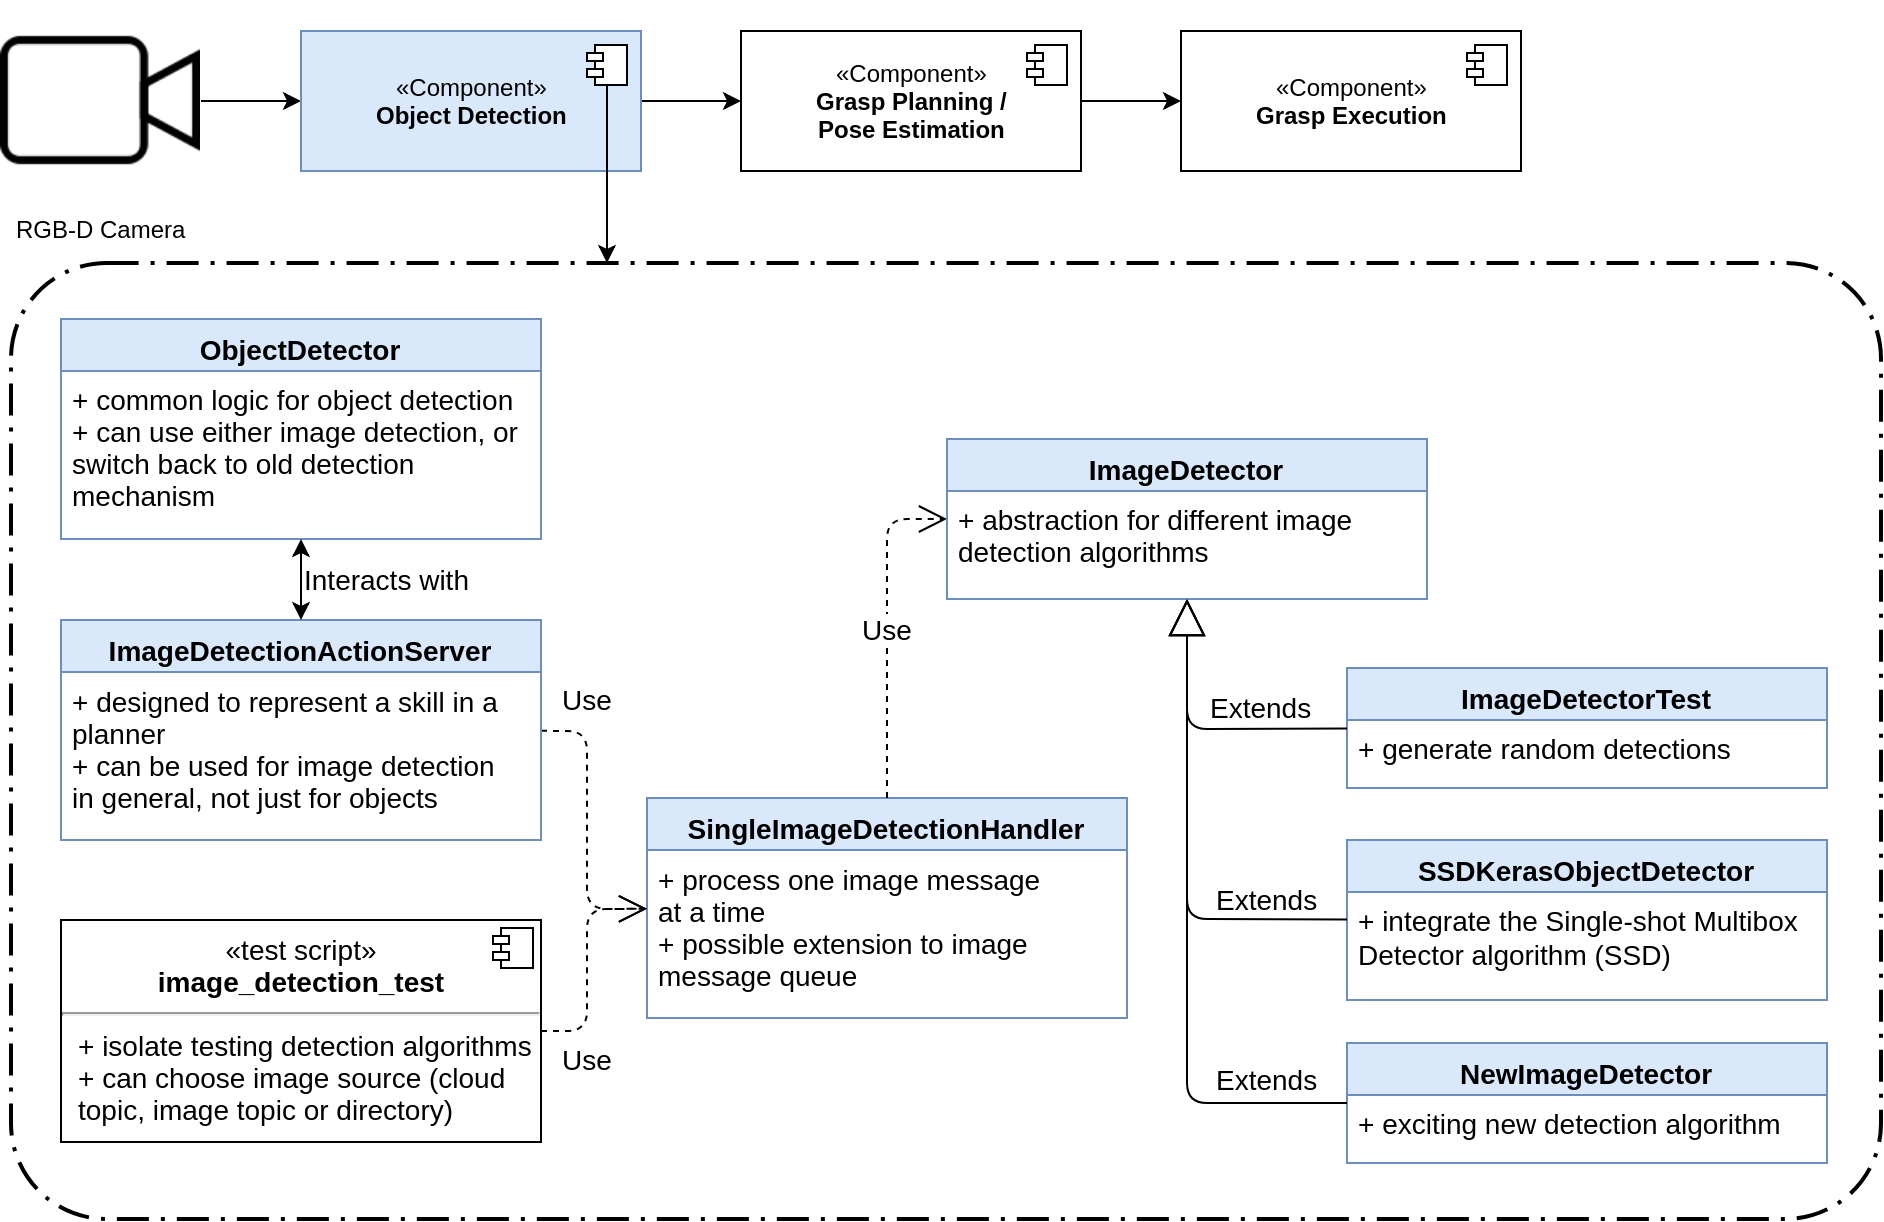
\includegraphics[width=0.95\linewidth]{grasp_pipeline_new_perception}
    \end{figure}
\end{frame}

\begin{frame}{Grasping software pipeline}
    \framesubtitle{Object detection -- Single Shot MultiBox Detector}
    \begin{figure}[b]
        \centering
        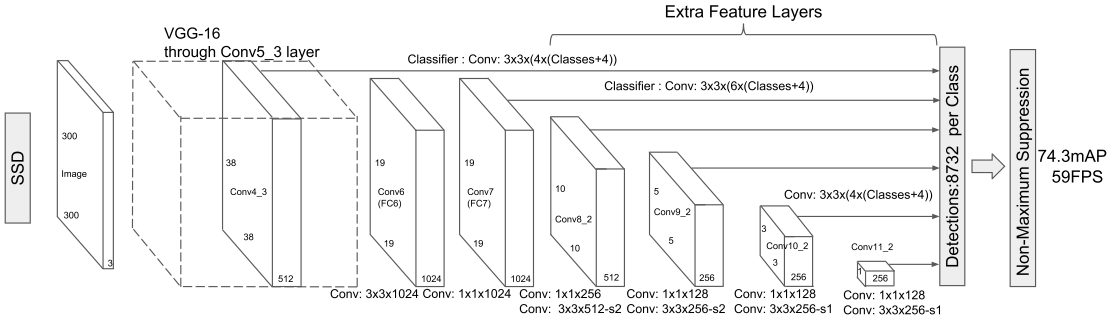
\includegraphics[width=0.8\linewidth]{liu_et_al-2016-ssd_arch}
        \caption{SSD architecture \cite{Liu2016SSD}.}
        \label{fig:ssd_arch}
    \end{figure}
    \begin{itemize}
        \item learns to adjust a set of default boxes to the ground truth bounding boxes
        \item learning at different scales are simulated by training different resolutions of the feature map
    \end{itemize}
\end{frame}

%%%%%%%%%%%%%%%%%%%%%
\begin{frame}{Grasping software pipeline}
    \framesubtitle{Grasp planning -- Object pose estimation}
    \begin{figure}[b]
        \centering
        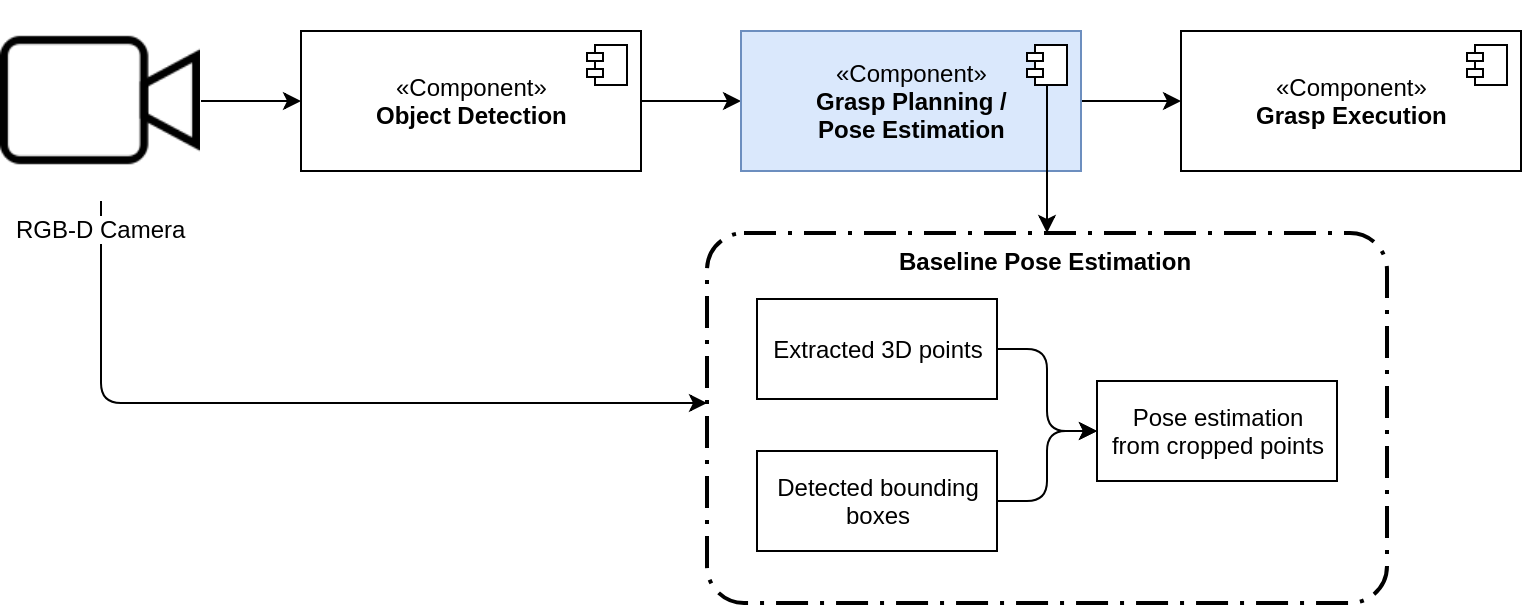
\includegraphics[width=0.7\linewidth]{grasp_pipeline_pose_estimation}
    \end{figure}
    \begin{columns}[onlytextwidth]
        \column{.6\textwidth}
        \scriptsize
        \begin{equation} \label{eq:pose_estimation_min}
        p = \left( \begin{matrix} x \\ y \\ z \end{matrix} \right) =
            \left( \begin{matrix}
                \min_{i = 1}^M B_{i,1} \\
                \cfrac{1}{M} \sum_{i = 1}^{M} B_{i,2} \\
                \cfrac{1}{M} \sum_{i = 1}^{M} B_{i,3}
            \end{matrix} \right)
        \end{equation}
        \begin{equation} \label{eq:pose_estimation_mean}
            p_j = \cfrac{1}{M} \sum_{i = 1}^{M} B_{i,j}
        \end{equation}
        \normalsize
        \column{.35\textwidth}
        \begin{figure}[b]
            \includegraphics<1->[width=0.7\textwidth]{base_link_frame}
            \caption{\texttt{base\_link} coordinate frame.}
        \end{figure}
    \end{columns}
\end{frame}

\begin{frame}{Grasping software pipeline}
    \framesubtitle{Grasp planning -- GQCNN}
    \begin{figure}[b]
        \centering
        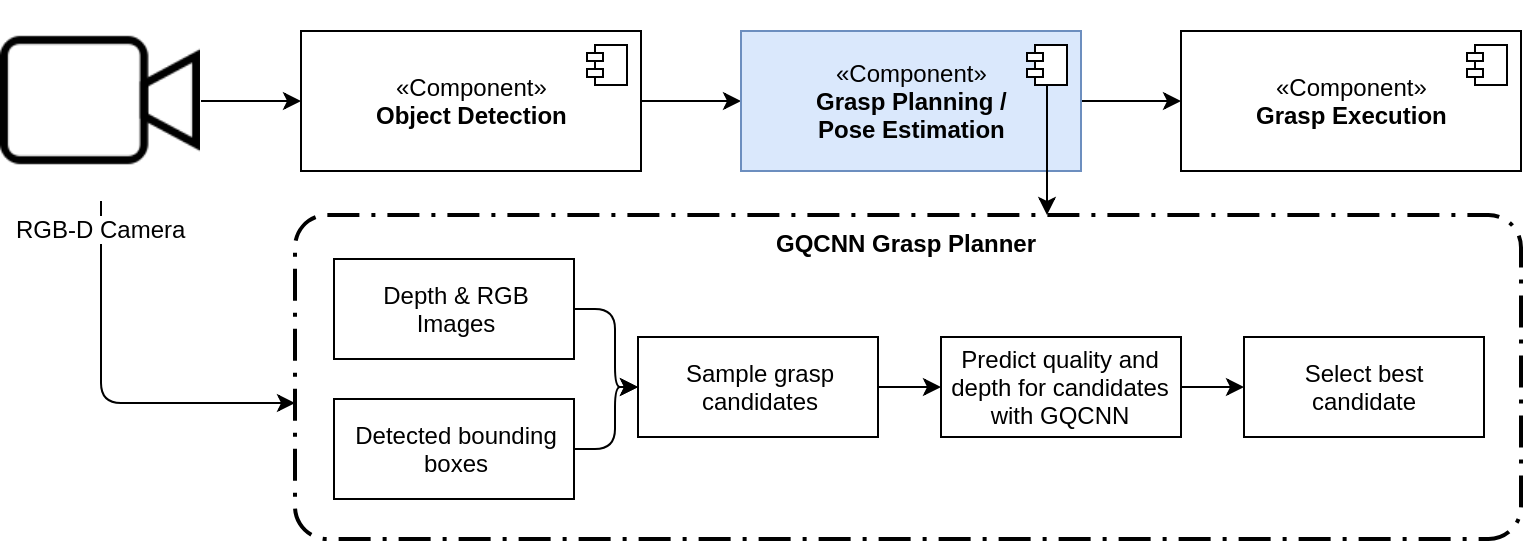
\includegraphics[width=0.8\linewidth]{grasp_pipeline_gqcnn}
    \end{figure}
\begin{exampleblock}{Issues}
    \begin{itemize}
        \item Assumpution of top-down camera view makes the depth prediction inaccurate
        \item Planned grasps take too long to calculate and are highly variant in depth
    \end{itemize}
\end{exampleblock}
\end{frame}

\begin{frame}{Grasping software pipeline}
\framesubtitle{Grasp planning -- GQCNN}%
    \begin{figure}[b]
    \centering
    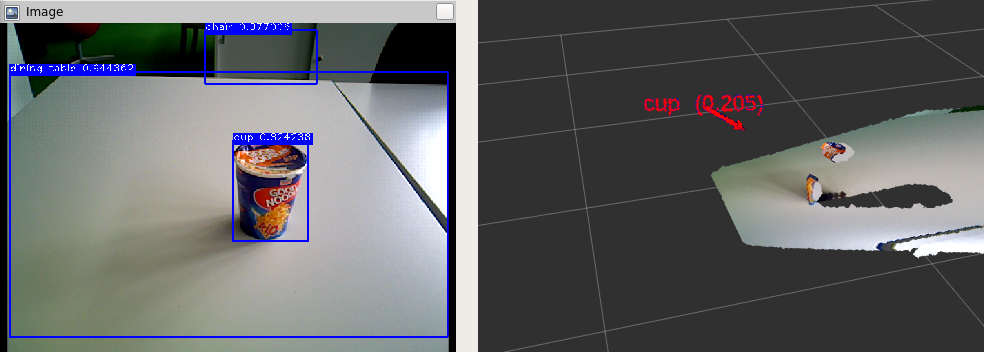
\includegraphics[width=0.9\linewidth]{grasp_gqcnn_result}
    \caption{\small A successful GQCNN grasp plan which took 40 seconds. Arrow and number on the right indicate grasp
        pose and quality returned from the GQCNN planner.}
    \label{fig:gqcnn_result}
    \end{figure}
\end{frame}

%%%%%%%%%%%%%%%%%%%%%
\begin{frame}{Grasping software pipeline}
    \framesubtitle{Grasp execution -- Dynamic Motion Primitives (DMP)}
    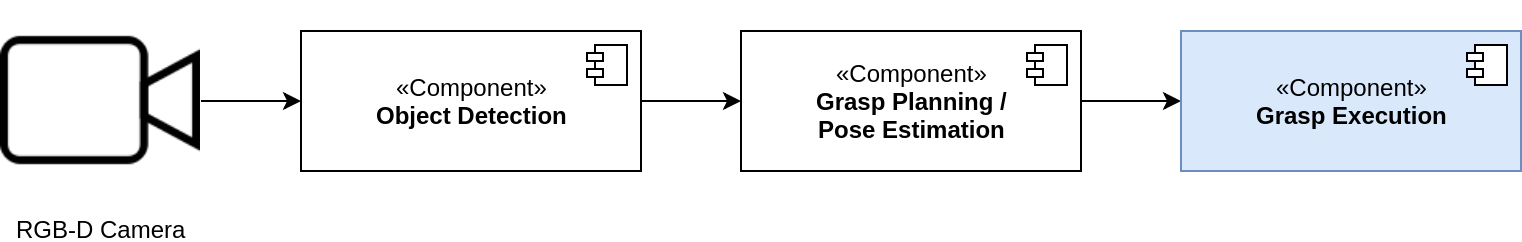
\includegraphics[width=\linewidth]{grasp_pipeline_execution}
    \begin{itemize}
        \item Manipulation planning uses the integration and extension of the DMP in a parallel project
            \cite{Padalkar2018}
        \item Model human-demonstrated trajectories as a series of differential equations
        \item Robot learns to perform similar movements via the solutions to these equations
    \end{itemize}
\end{frame}

%%%%%%%%%%%%%%%%%%%%%%%%%%%%%%%%%%%%%%%%%
\section{Experiments}
\begin{frame}{Experiments}
\framesubtitle{Setup}
    \begin{columns}[onlytextwidth]
        \column{.6\textwidth}
        \begin{itemize}
            \footnotesize
            \item 20 grasp attempts for each variances of the baseline method
            \item Predefined starting position for each attempt as seen in figure \ref{fig:exp_setup}
            \item Arm collisions and object slips are counted as failures
            \item Only one of the objects in figure \ref{fig:objects} is grasped at a time
        \end{itemize}
        \column{.35\textwidth}
        \begin{figure}[b]
            \includegraphics<1->[width=\textwidth]{experimental_setup}
            \caption{\small Robot at initial position.}
            \label{fig:exp_setup}
        \end{figure}
    \end{columns}
\end{frame}

\begin{frame}{Experiments}
\framesubtitle{Objects}%
\begin{figure}[t]
    \centering
    \begin{subfigure}[t]{0.23\textwidth}
        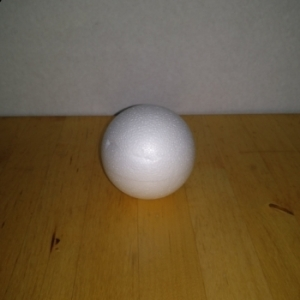
\includegraphics[width=\textwidth]{object_ball}
        \caption{\scriptsize Styrofoam ball}
        \label{fig:object_ball}
    \end{subfigure}
    ~
    \begin{subfigure}[t]{0.23\textwidth}
        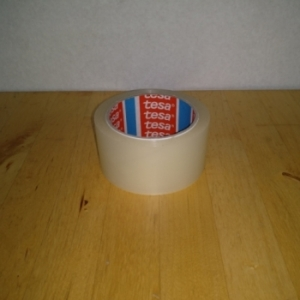
\includegraphics[width=\textwidth]{object_duct_tape}
        \caption{\scriptsize Duct tape}
        \label{fig:object_duct_tape}
    \end{subfigure}
    ~
    \begin{subfigure}[t]{0.23\textwidth}
        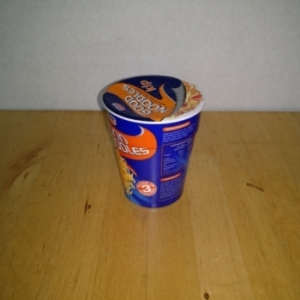
\includegraphics[width=\textwidth]{object_noodle_box}
        \caption{\scriptsize Noodles box}
        \label{fig:object_noodle_box}
    \end{subfigure}
    ~
    \begin{subfigure}[t]{0.23\textwidth}
        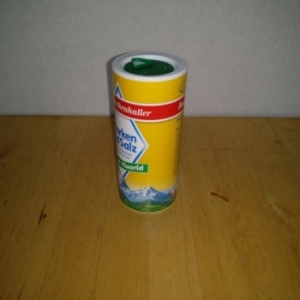
\includegraphics[width=\textwidth]{object_salt}
        \caption{\scriptsize Salt container}
        \label{fig:object_salt}
    \end{subfigure}
    \caption{Objects selected for the experiments.}\label{fig:objects}
\end{figure}
\end{frame}

\begin{frame}{Experiments}
\framesubtitle{Results}
\begin{table}[h!]
    \small
    \begin{tabularx}{\textwidth}{L{0.2\textwidth}C{0.15\textwidth}C{0.15\textwidth}C{0.15\textwidth}C{0.15\textwidth}}
        \cmidrule[0.08em](){1-5}
        \multirow{2}{*}{Object} & \multicolumn{2}{c}{Mean $ x $} & \multicolumn{2}{c}{Minimum $ x $}    \\
        \cmidrule[0.08em](){2-5}
                                & Success   & Failure               & Success   & Failure               \\
        \cmidrule[0.08em](){1-5}
        Salt                    & 17        & 3                     & 16        & 4                     \\
        Ball                    & 8         & 12                    & 15        & 5                     \\
        Noodle box              & 16        & 4                     & 12        & 8                     \\
        Duct tape               & 7         & 13                    & 13        & 7                     \\
        \cmidrule[0.08em](){1-5}
    \end{tabularx}
    \caption{Counts of successful and failed grasp attempts during the experiments. ``Mean $ x $'' and
        ``Minimum $ x $''  refer to the two baseline pose estimation methods which, respectivly, use the mean and
        minimum object coordinates along the $ x $-axis to estimate the grasp pose
        \footnote{A video of a complete experiment for one object is available on YouTube at
        \url{https://youtu.be/OC7vttt4-Jo}}.}
    \label{table:grasp_exp_result}
\end{table}
\end{frame}

\begin{frame}{Experiments}
\framesubtitle{Discussion}%
    \begin{figure}[t]
    \centering
    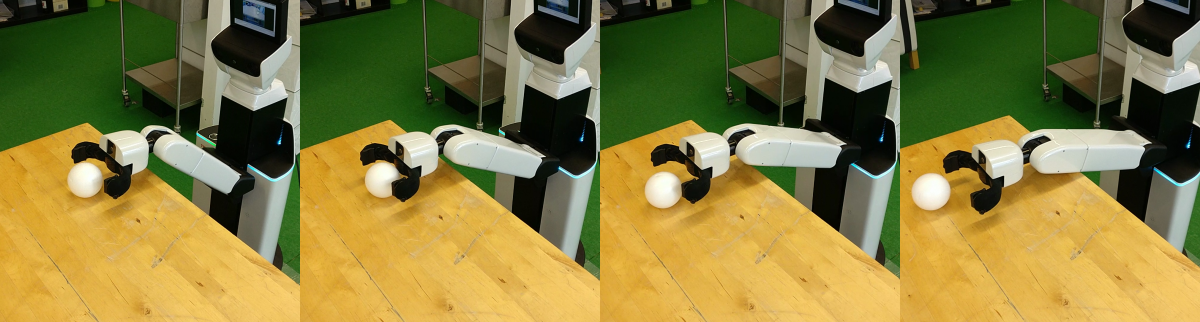
\includegraphics[width=0.8\linewidth]{grasp_ball_fail}
    \caption{\small The gripper pushes on the ball and it rolls forward}
    \label{fig:grasp_ball_fail}
    \end{figure}
    \begin{itemize}
        \small
        \item Grasping the ball using the Minimum $ x $ method is better since the arm doesn't push it forward
        \item Low, hollow objects like duct tape give low $ z $ estimates, which suggest that a top-down grasp may
        perform better
        \item Slippage can be avoided by utilizing the gripper's force sensors.
    \end{itemize}
\end{frame}

%%%%%%%%%%%%%%%%%%%%%%%%%%%%%%%%%%%%%%%%%
\begin{frame}{Conclusions}
\scriptsize
\begin{exampleblock}{Contributions}<1->
    \begin{itemize}
        \item Design and implementation of an object detection architecture which is compatible with old methods while
        flexible to new detection algorithms
        \item Implementation of a grasping pipeline (in conjunction with \cite{Padalkar2018}) reliable enough to
            perform hudreds of grasps in succession, enabling evaluation of more advanced approaches in the future
    \end{itemize}
\end{exampleblock}
\begin{exampleblock}{Future works}<2->
    \begin{itemize}
        \item More advanced and reliable methods can be experimented in place for GQCNN
        \item Incorporating the force sensor and hand camera would provide much more information for grasp planning,
            and may produce more robust grasps
    \end{itemize}
\end{exampleblock}
\normalsize
\end{frame}

\begin{frame}{}
\begin{center}
    \Huge \emph{Questions}
\end{center}
\end{frame}

%%%%%%%%%%%%%%%%%%%%%%%%%%%%%%%%%%%%%%%%
\begin{frame}[allowframebreaks]{References}
    \printbibliography
\end{frame}

\end{document}
